\subsection{Energy-Based Models and Boltzmann Machines \cite{Bengio2009}}

In this survey we present the fifth chapter of the book \emph{Learning Deep Architectures for AI} by Bengio \cite{Bengio2009}. This chapter introduces the main mathematical concepts helpful to understand \emph{Restricted Boltzmann Machines (RBMs)}, which are particular energy-based models.

Energy-based models associate a scalar energy to each configuration of the variables of interest. For example, we would like plausible or desirable configurations to have low energy. The probability distribution of an energy-based model may be defined as follows:
\begin{equation}\label{equ:1}
P(x) = \frac{e^{-Energy(x)}}{Z}.
\end{equation}
Here $Z$ is a normalization term called the \emph{partition function} by analogy with physical systems.

In the \emph{products of experts} formulation, the energy function is a sum of terms, each one associated with an ``expert'' $f_i$:
\begin{equation}
Energy(x) = \sum_i f_i(x).
\end{equation}
Each expert can thus be seen as a detector of implausible configurations of $x$, or equivalently, as enforcing constraints on $x$.

In many cases we do not observe all the components simultaneously, or we want to introduce some non-observed variables to increase the expressive power of the model. So we consider an observed part $x$ and a hidden part $h$:
\begin{eqnarray}
P(x,h) = \frac{e^{-Energy(x,h)}}{Z},\\
P(x) = \sum_h P(x,h).
\end{eqnarray}
In order to map this formulation to the standard form, we introduce the notation of \emph{free energy}:
\begin{eqnarray}
P(x) = \frac{e^{-FreeEnergy(x)}}{Z},\\
FreeEnergy(x) = - \log \sum_h e^{-Energy(x,h)}.
\end{eqnarray}

The average log-likelihood gradient over the training set is
\begin{eqnarray}
E_{\hat{P}}[\frac{\partial \log P(x)}{\partial \theta}] = - E_{\hat{P}}[\frac{\partial FreeEnergy(x)}{\partial \theta}] + E_P[\frac{\partial FreeEnergy(x)}{\partial\theta}],
\end{eqnarray}
where expectations are over $x$, with $\hat{P}$ the training set empirical distribution and $E_P$ the expectation under the model's distribution.

If the energy can be written as a sum of terms associated with at most one hidden unit:
\begin{eqnarray}
Energy(x,h) = -\beta(x) + \sum_i \gamma_i(x, h_i),
\end{eqnarray}
then the free energy and numerator of the likelihood can be computed tractably:
\begin{eqnarray}
P(x) = \frac{e^\beta(x)}{Z} \prod_i \sum_{h_i} e^{-\gamma_i(x, h_i)}.
\end{eqnarray}

The \emph{Boltzmann machine} is a particular type of energy-based model with hidden variables. In a Boltzmann machine, the energy function is a general second-order polynomial:
\begin{eqnarray}
Energy(x,h) = -b'x - c'h - h'Wx - x'Ux - h'Vh.
\end{eqnarray}
The gradient of the log-likelihood can be written as:
\begin{eqnarray}
\frac{\partial \log P(x)}{\partial \theta} = - \sum_h P(h|x) \frac{\partial Energy(x,h)}{\partial \theta} + \sum_{\hat{x},h} P(\hat{x}, h) \frac{\partial Energy(\hat{x},h)}{\partial \theta}.
\end{eqnarray}
This gradient can be computed, if we have a procedure to sample from $P(h|x)$ and from $P(x,h)$. The basic idea is to use \emph{Gibbs sampling} in two phases: in the \emph{positive phase}, $x$ is clamped to the observed input vector, and we sample $h$ given $x$; in the \emph{negative phase} both $x$ and $h$ are sampled. Since two \emph{MCMCs (Monte Carlo Markov Chain)} (one for the positive phase and one for the negative phase) are needed for each example $x$, the computation can be very expensive.

\begin{figure}[h]
  \centering
  % Requires \usepackage{graphicx}
  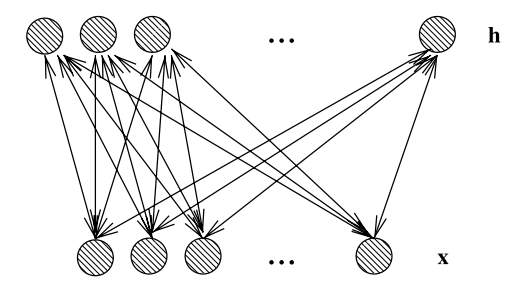
\includegraphics[width=.6\linewidth]{Bengio09-RBM.png}\\
  \caption{Undirected graphical model of a RBM}\label{fig:Bengio09}
\end{figure}

In the \emph{Restricted Boltzmann Machine (RBM)}, the $h_i$ are independent of each other when conditioning on $x$, and the $x_j$ are independent of each other when conditioning on $h$ (cf. Figure \ref{fig:Bengio09}). The energy function is bilinear:
\begin{eqnarray}
Energy(x,h) = -b'x - c'h - h'Wx.
\end{eqnarray}
The free energy of the input can be computed efficiently:
\begin{eqnarray}
FreeEnergy(x,h) = -b'x - \sum_i \log \sum_{h_i} e^{h_i(ci + W_i x)}.
\end{eqnarray}
Using the same factorization trick, we can obtain a tractable expression for $P(h|x)$ and $P(x|h)$.

Gibbs sampling in fully connected Boltzmann Machines is slow because there are as many sub-steps in the Gibbs chain as there are units in the network. The Factorization enjoyed by RBMs bring two benefits: 1) we do not need to sample in the positive phase because the free energy is computed analytically; 2) the set of variables $(x,h)$ can be sampled in two sub-steps in each step of the Gibbs chain: first we sample $h$ given $x$, and then a new $x$ given $h$.

\emph{Contrastive Divergence (CD)} is an approximation of the log-likelihood gradient that has been found to be a successful update rule for training RBMs. The basic idea of $k$-step CD is simple, and involves a second approximation, which introduces some bias in the gradient: run the MCMC chain $x_1, ..., x_{k+1}$ for only $k$ steps starting from the observed example $x_1 = x$. The surprising empirical result is that even $k=1$ often gives good results.

